\documentclass[oneside,pdflatex,sn-mathphys-num]{sn-jnl}

\usepackage{graphicx}
\usepackage{multirow}
\usepackage{amsmath,amssymb,amsfonts}
\usepackage{textcomp}
\usepackage{booktabs}
\usepackage{subcaption}

\makeatletter
\@twosidefalse
\@mparswitchfalse
\makeatother
\geometry{
  paperwidth=210mm,
  paperheight=297mm,
  top=26mm,
  headheight=5.5pt,
  headsep=5.6mm,
  textheight=194.25mm,
  left=39.41mm,
  right=39.41mm,
  marginparsep=0mm,
  marginparwidth=0mm,
  bindingoffset=0mm
}

\flushbottom

\begin{document}

\title[BAMNet for TAVI Guidance]{BoundaryAwareMAnet: Multi-Task Fluoroscopic Segmentation of the Aortic Root and Landmark Localization for TAVI Guidance}

\author*[1]{\fnm{Nikita V.} \sur{Laptev}}\email{nikitalaptev77@gmail.com}

\author[2]{\fnm{Olga M.} \sur{Gerget}}

\author[3]{\fnm{Julia K.} \sur{Belova}}

\author[1]{\fnm{Evgeny E.} \sur{Vasilchenko}}

\author[3]{\fnm{Mikhail A.} \sur{Chernyavsky}}

\author*[4]{\fnm{Viacheslav V.} \sur{Danilov}}\email{viacheslav.v.danilov@gmail.com}

\affil*[1]{\orgname{Siberian State Medical University}, \orgaddress{\city{Tomsk}, \country{Russia}}}

\affil[2]{\orgname{Institute of Control Sciences of Russian Academy of Sciences}, \orgaddress{\city{Moscow}, \country{Russia}}}

\affil[3]{\orgname{Almazov National Medical Research Center}, \orgaddress{\city{Saint Petersburg}, \country{Russia}}}

\affil[4]{\orgname{Pompeu Fabra University}, \orgaddress{\city{Barcelona}, \country{Spain}}}

\abstract{Accurate intraoperative visualization of the aortic root during transcatheter aortic valve implantation (TAVI) is essential for safe valve positioning, yet fluoroscopy remains challenging because of low soft-tissue contrast, motion artifacts, and occlusion by endovascular devices. Repeated contrast injections further increase the risk of renal complications, particularly in patients with pre-existing chronic kidney disease. We present BoundaryAwareMAnet (BAMNet), a multitask neural network for simultaneous aortic root segmentation and localization of four key anatomical landmarks on fluoroscopic images. The model combines an EfficientNet-V2 encoder, a modified MA-Net decoder with global spatial attention, a dedicated landmark head with coordinate-aware feature modulation and heatmap prediction, and an auxiliary boundary pathway used for boundary-guided supervision. The study used 2,925 grayscale intraoperative images from 83 patients. On the validation set, BAMNet achieved a Dice score of 0.887, an IoU of 0.805, and a mean landmark localization error of 3.16~mm (11.95~px) while preserving real-time performance at 43.9 FPS. In patient-level 5-fold cross-validation, the model achieved a Dice score of $0.897 \pm 0.024$ and a mean localization error of $11.13 \pm 0.76$~px. These findings indicate that joint segmentation and landmark localization on fluoroscopy is feasible and may provide a practical foundation for contrast-sparing visual guidance and future robot-assisted TAVI systems.}

\keywords{TAVI, aortic root segmentation, landmark localization, multitask learning, fluoroscopy}

\maketitle

\section{Introduction}\label{sec:introduction}

Aortic stenosis remains one of the most common and clinically important valvular diseases in aging populations worldwide. As life expectancy increases, the number of patients with severe aortic stenosis also continues to rise. Transcatheter aortic valve implantation (TAVI) has become a major interventional treatment option in contemporary cardiology, with expanding indications in patients at intermediate and low surgical risk \cite{otto2020_guideline,vahanian2021_guidelines,leon2019_partner3}.

Despite this expansion, optimal valve positioning during deployment remains a major determinant of procedural success and long-term outcome. Suboptimal implantation depth and alignment relative to the annular plane and coronary ostia may increase the risk of paravalvular regurgitation, coronary obstruction, or conduction disturbances requiring permanent pacemaker implantation \cite{pibarot2021_pvl,jilaihawi2022_coronary,kammler2016_implantdepth}. Accurate real-time visualization is therefore central to safe guidance.

In current clinical practice, operators rely primarily on fluoroscopy, often supplemented by repeated contrast aortography to delineate the aortic root, annular plane, and coronary ostia. Fluoroscopy offers high temporal resolution, but it also suffers from low soft-tissue contrast, noise, respiratory and cardiac motion, and frequent occlusion by guidewires, catheters, and delivery systems. These limitations increase dependence on contrast administration and operator experience. Hybrid approaches based on preoperative CT and CT-fluoroscopy fusion have been explored for procedural guidance, but their accuracy may be limited by cardiorespiratory motion, deformation from stiff guidewires, and the lack of continuous real-time updating during valve deployment \cite{vernikouskaya2017_imageguidance,vernikouskaya2018_registration}.

In our previous work, we performed a large-scale comparison of six modern convolutional architectures for automatic aortic root segmentation on intraoperative TAVI frames. On a dataset of 2,925 images from 83 patients with strict patient-level 5-fold cross-validation, the best single-task model, MA-Net with an EfficientNet-B4 encoder, achieved a median Dice score of 0.942 and an ASSD of 4.07~mm \cite{laptev2025_aorticroot}. These results showed that high-quality segmentation is possible even under low-contrast fluoroscopic conditions. However, a segmentation mask alone is insufficient when sub-pixel landmark coordinates are needed for automated or robotic valve positioning.

The next stage in TAVI guidance is the transition toward robot-assisted and potentially autonomous delivery platforms. Early translational robotic systems are already emerging, including AI-guided positioning studies and the ongoing feasibility evaluation of the TAVIPILOT platform \cite{smits2025_autonomous,clinicaltrials_nct07152574}. Such systems require not only a contour of the aortic root, but also reliable and temporally stable localization of key landmarks, especially the two annular points (AA1 and AA2) and the two sinotubular-junction landmarks near the coronary ostia (STJ1 and STJ2).

To address this clinical and technological need, we developed BoundaryAwareMAnet (BAMNet), a multitask architecture designed for simultaneous aortic root segmentation and precise localization of four landmarks on intraoperative fluoroscopic images. We hypothesized that combining global contextual reasoning, coordinate-aware feature modulation, and explicit boundary-focused supervision in a unified multitask formulation would improve both segmentation quality and landmark localization performance.

\section{Materials and Methods}\label{sec:methods}

\subsection{Dataset and annotation protocol}\label{subsec:dataset}

The study used intraoperative fluoroscopic images acquired during TAVI procedures in patients with severe aortic stenosis. The present work builds on a previously published dataset of intraoperative angiographic images and extends it with additional patients and revised annotations. The final dataset comprised 2,925 grayscale images of size $1000 \times 1000$ pixels (8-bit) obtained from 83 patients between 2018 and 2024.

The primary annotation task was binary segmentation of the aortic root. The expert mask represented the visible contour of the contrast-enhanced aortic root in the current frame. Guidewires, catheters, valve delivery system components, and other radiopaque instruments were deliberately excluded from the mask. Annotation was performed in the Supervisely web-based computer vision platform, consistent with the previous dataset release (Fig.~\ref{fig:annotation_examples}).

\begin{figure}[htbp]
    \centering
    \begin{subfigure}[b]{0.48\textwidth}
        \centering
        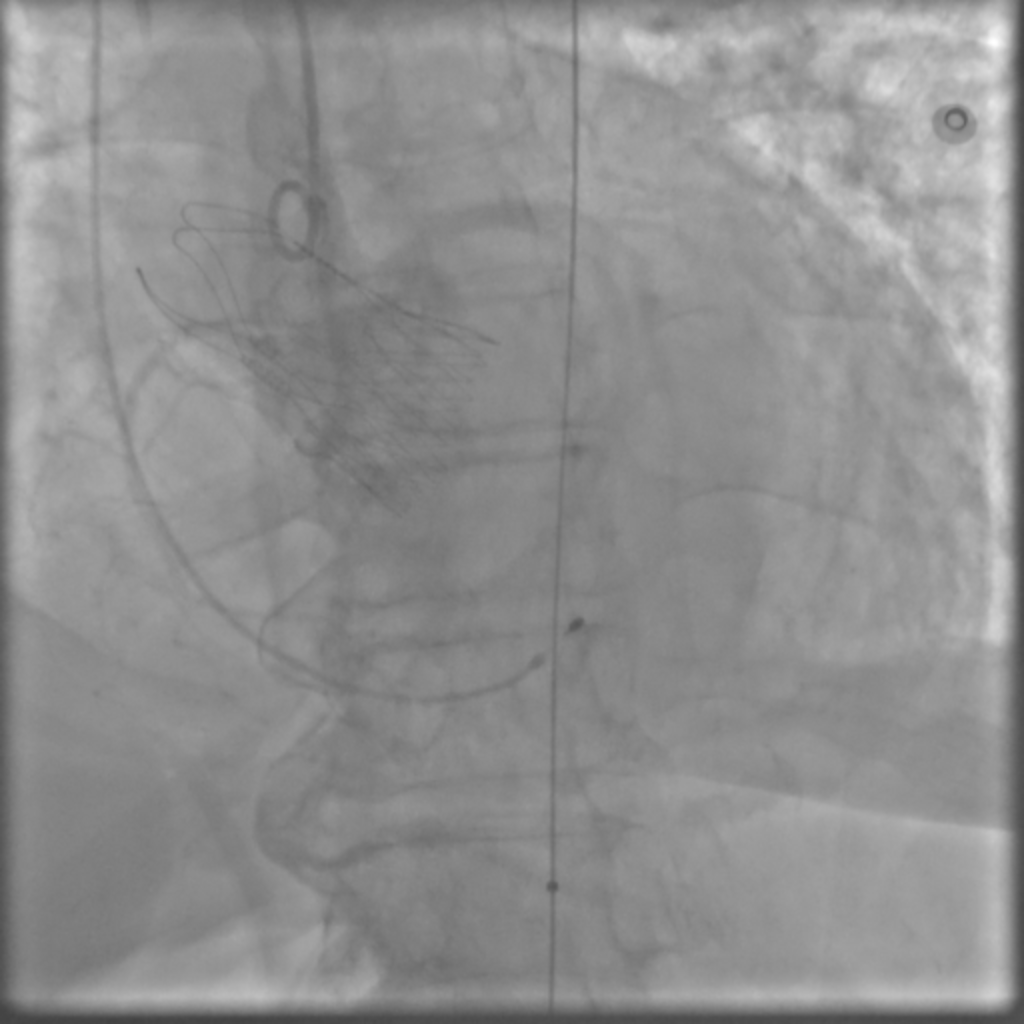
\includegraphics[width=\textwidth]{../fgure_article/orig_15_0025_004_029.png}
        \caption{}
        \label{fig:orig1}
    \end{subfigure}
    \hfill
    \begin{subfigure}[b]{0.48\textwidth}
        \centering
        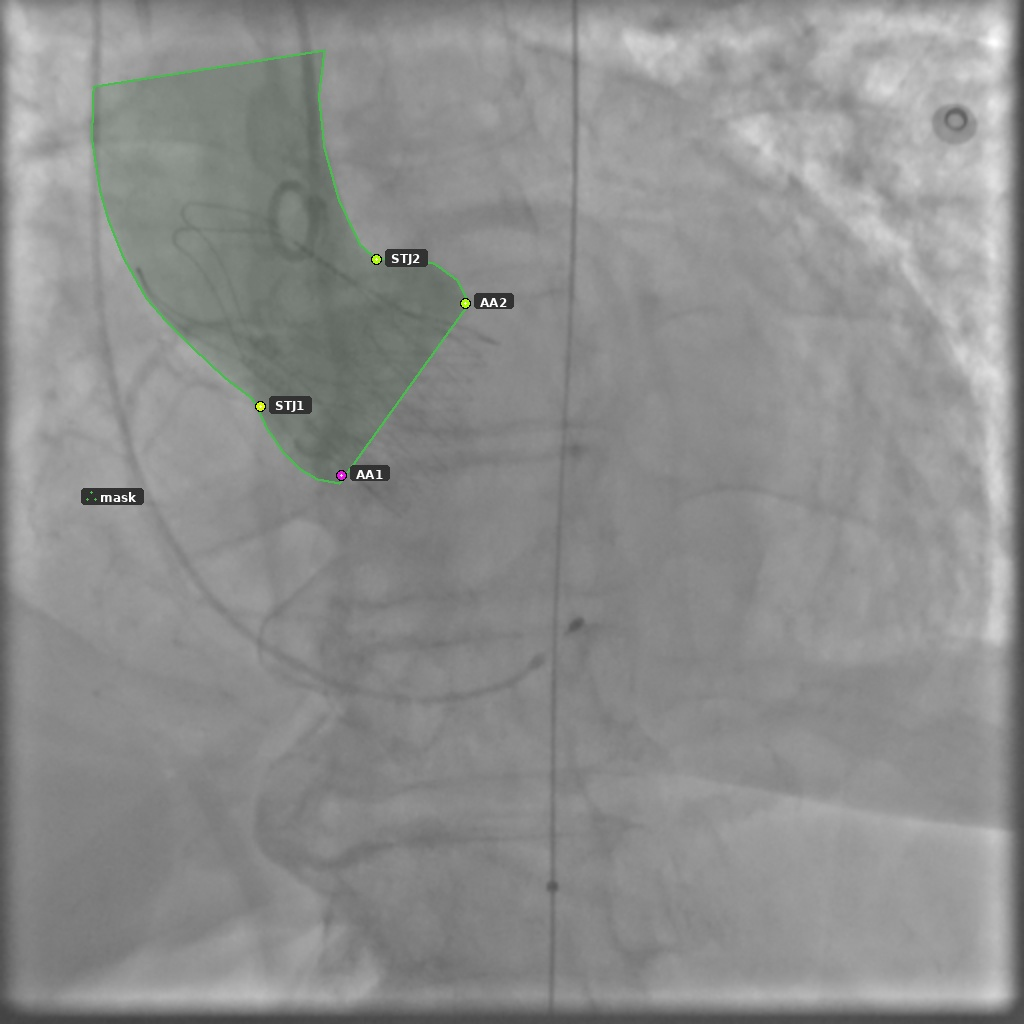
\includegraphics[width=\textwidth]{../fgure_article/sample_15_0025_004_029.jpeg}
        \caption{}
        \label{fig:annot1}
    \end{subfigure}
    \vskip\baselineskip
    \begin{subfigure}[b]{0.48\textwidth}
        \centering
        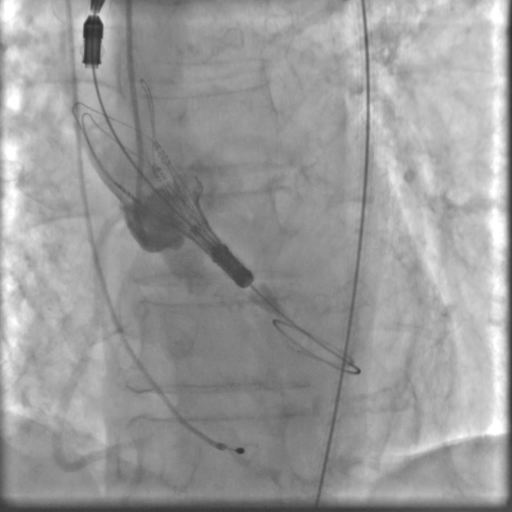
\includegraphics[width=\textwidth]{../fgure_article/orig_19_0019_008_031.png}
        \caption{}
        \label{fig:orig2}
    \end{subfigure}
    \hfill
    \begin{subfigure}[b]{0.48\textwidth}
        \centering
        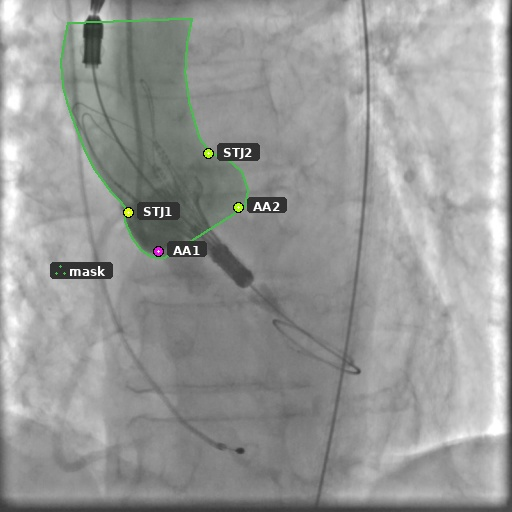
\includegraphics[width=\textwidth]{../fgure_article/sample_19_0019_008_031.jpeg}
        \caption{}
        \label{fig:annot2}
    \end{subfigure}
    \caption{Representative fluoroscopic images (a, c) and corresponding expert annotations (b, d) illustrating the aortic root mask and four anatomical landmarks (AA1, AA2, STJ1, STJ2).}
    \label{fig:annotation_examples}
\end{figure}

In addition to binary masks, each image was annotated with four key anatomical landmarks: two points on the aortic annulus (AA1 and AA2) and two landmarks near the coronary ostia at the sinotubular junction (STJ1 and STJ2). For each landmark, two-dimensional coordinates $(x,y)$ and a binary visibility flag were stored. A landmark was considered visible only when its position could be identified reliably on the current frame. When anatomy was obscured by devices, contrast opacification was insufficient, or the anatomical configuration was ambiguous, the landmark was marked as invisible.

To assess generalization properly, all experiments followed a patient-level protocol that prevented frames from the same patient from appearing in both training and validation/test subsets. Five-fold patient-level cross-validation was used throughout. In each fold, approximately 86--88\% of patients were assigned to training and 12--14\% to validation/test. Because the number of frames per patient varied, the exact image counts differed slightly across folds.

\subsection{Training strategy}\label{subsec:training}

Before model input, all images were resized to a fixed resolution of $640 \times 640$ pixels. Original single-channel fluoroscopic frames were converted to a three-channel representation by channel duplication so that an ImageNet-pretrained encoder could be used. Images were then standardized with ImageNet mean and standard deviation values. Segmentation masks were resized with nearest-neighbor interpolation to preserve binary structure. Landmark coordinates were recomputed after geometric transforms and normalized to the $[0,1]$ range.

Augmentations were applied only to the training subset and were implemented with custom transformations. Their purpose was both to enlarge the effective training distribution and to regularize the model against overfitting. The augmentation pipeline included horizontal flipping with probability 0.5, accompanied by mandatory swapping of landmark pairs AA1$\leftrightarrow$AA2 and STJ1$\leftrightarrow$STJ2; affine transforms with scaling in the range 0.85--1.15, rotations within $\pm 20^{\circ}$, translations up to $\pm 8$\% along each axis, and mild shear up to $\pm 5^{\circ}$; moderate elastic deformation; CLAHE-based local contrast enhancement; random brightness and contrast adjustment; gamma correction; additive Gaussian noise; Gaussian blur and motion blur; simulated illumination non-uniformity and vignetting; and coarse dropout to mimic partial occlusion by interventional tools. Vertical flipping was intentionally excluded because it is not anatomically plausible in this fluoroscopic setting. If a landmark moved outside the image after a geometric transform, its visibility flag was reset to zero.

Training was performed in PyTorch with PyTorch Lightning. AdamW was used as the optimizer with an initial learning rate of $5 \times 10^{-4}$ and weight decay of $3 \times 10^{-4}$. The learning rate was adapted with ReduceLROnPlateau using a validation balance score that combined segmentation quality and landmark localization accuracy. To stabilize optimization, several parameters were scheduled smoothly. The soft-argmax temperature increased during early epochs from $\beta=2$ to $\beta=12$, enabling a transition from smoother to more localized coordinate distributions. At the same time, the width of the Gaussian target heatmaps was gradually reduced so that training started from softer targets and then shifted toward higher spatial precision.

The contribution of the landmark branch and the influence of boundary-guided feature enhancement were also introduced progressively to avoid early optimization instability. In later epochs, the weight of the point-related loss component was reduced to improve the balance between segmentation quality and landmark localization.

\subsection{Proposed multitask architecture}\label{subsec:architecture}

BoundaryAwareMAnet (BAMNet) was designed as a single multitask network for simultaneous dense segmentation of the aortic root and localization of anatomical landmarks. Both tasks are solved in one forward pass, which is important for intraoperative deployment under real-time latency constraints.

The model is built on an ImageNet-pretrained EfficientNet-V2 encoder that extracts features at multiple spatial scales. These features are fused in a decoder inspired by U-Net and MA-Net so that the network can combine global anatomical context with local contour details. At low-resolution decoder levels, additional spatial attention is applied to improve reconstruction of the continuous aortic root contour in difficult frames affected by low contrast, noise, motion, and device overlap.

The segmentation branch produces two outputs:
\begin{enumerate}
\item binary segmentation logits for the aortic root;
\item an intermediate high-resolution feature representation that is reused by the landmark branch.
\end{enumerate}

The landmark branch receives fused features from the deepest encoder stage and the segmentation pathway. It consists of local convolutional processing and a Coordinate Attention module that preserves vertical and horizontal positional structure. The branch predicts landmark heatmaps, while a separate auxiliary boundary head operating on segmentation features produces a boundary-weight map. Boundary guidance is implemented by projecting segmentation features and injecting them into the landmark branch during training.

This design allows the model to exploit both global root morphology and local contour geometry when localizing landmarks. The complete architecture is shown in Fig.~\ref{fig:bamnet_architecture}.

\begin{figure}[htbp]
\centering
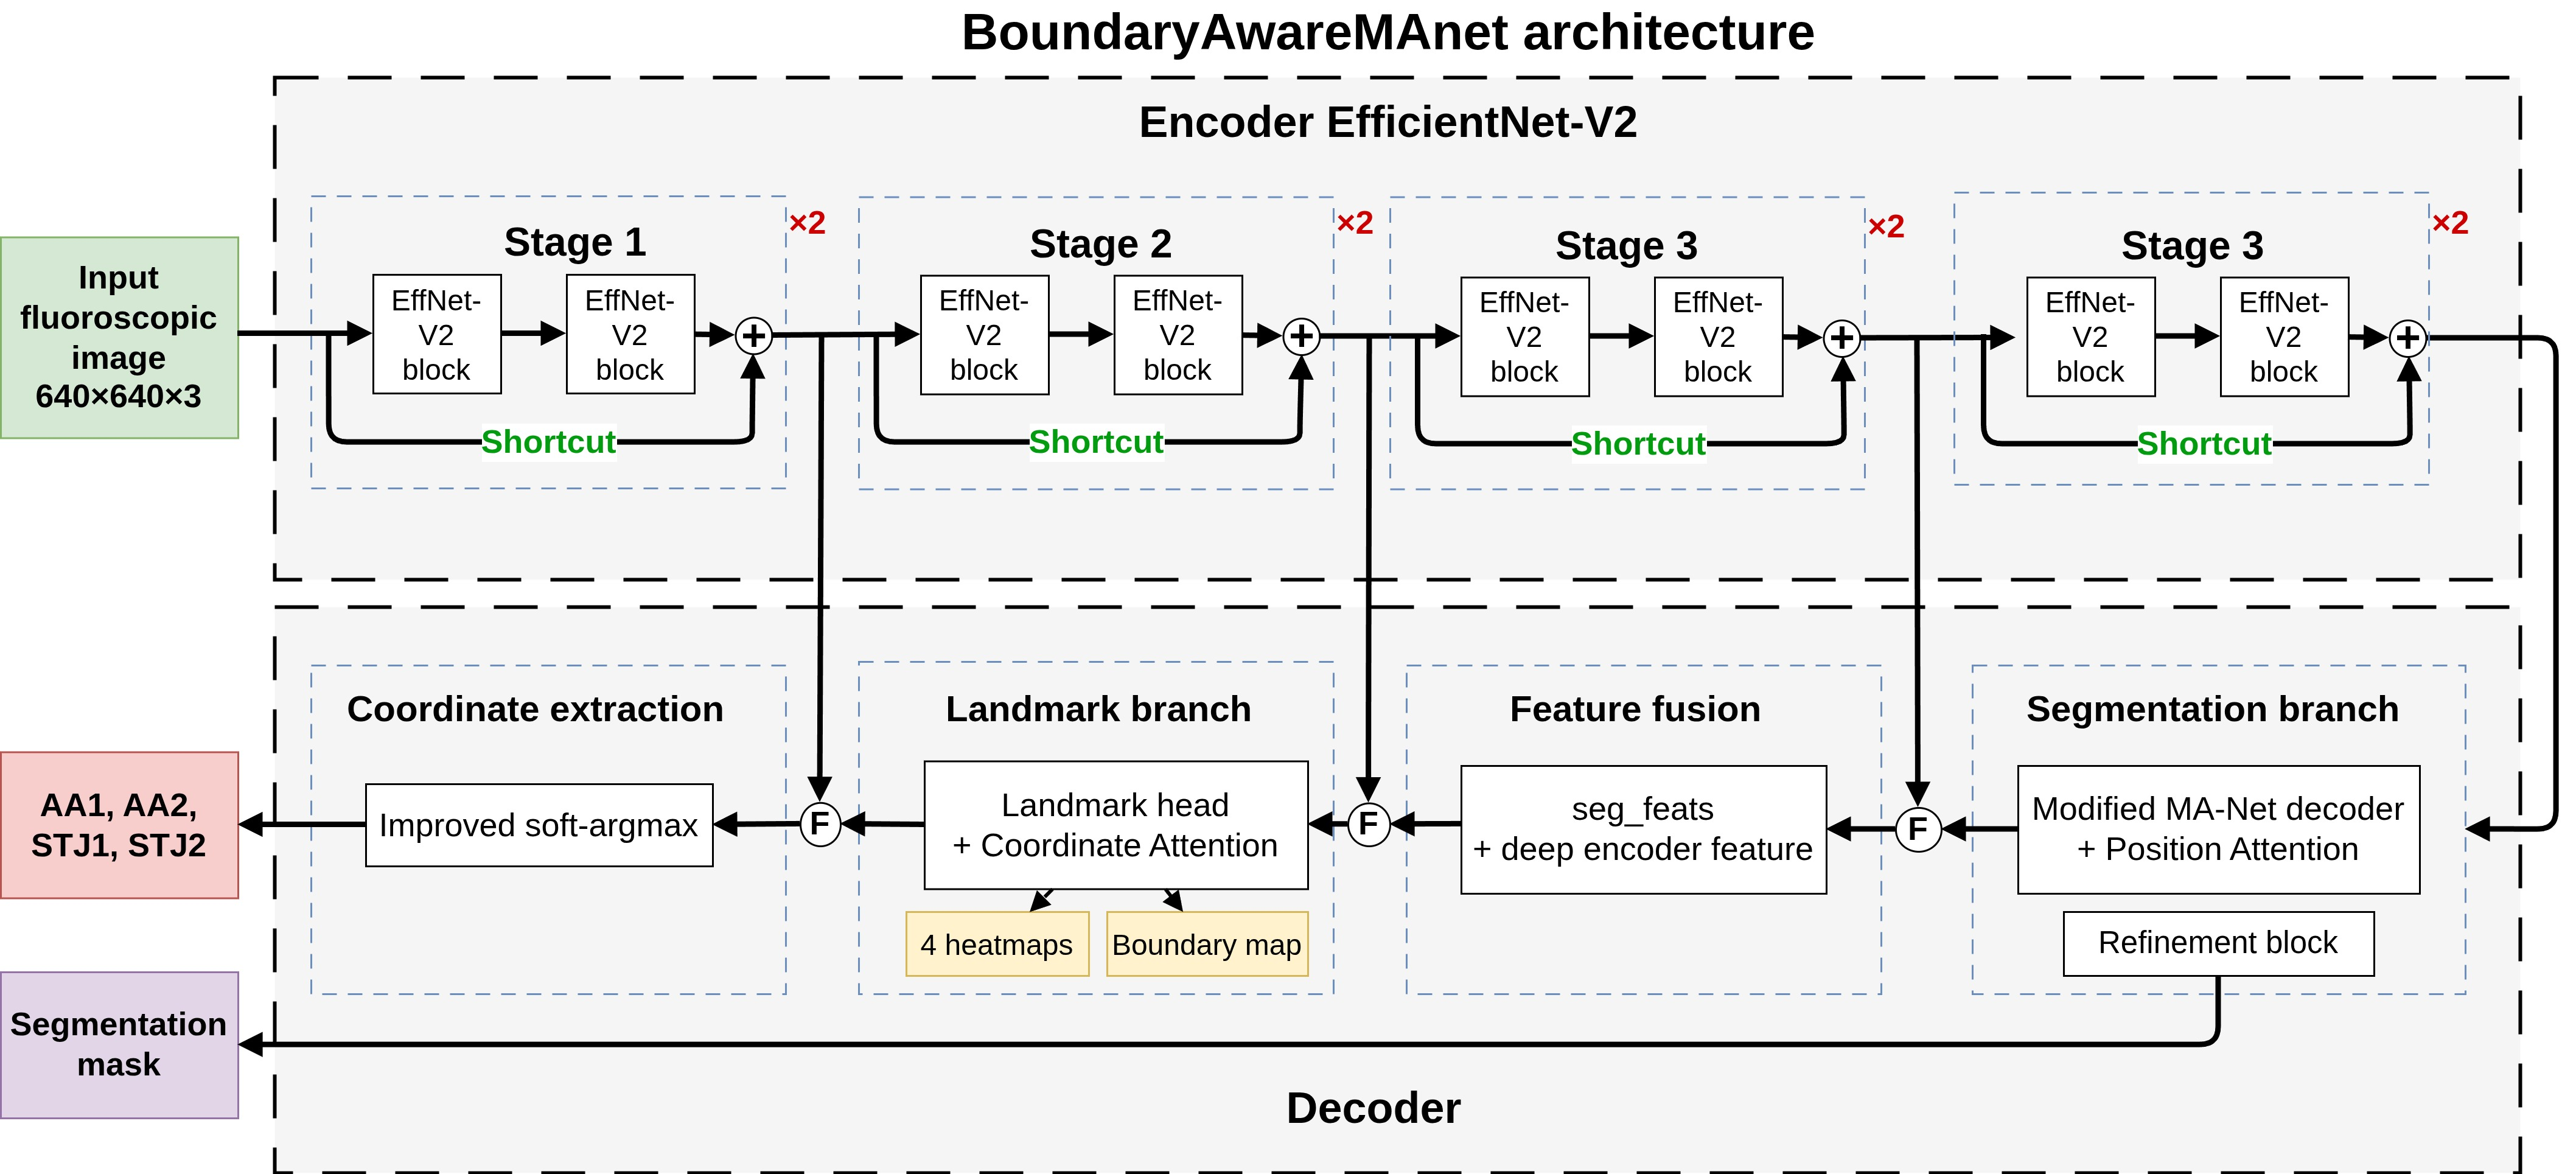
\includegraphics[width=\textwidth]{../fgure_article/figeure_orginal/BAMNet.jpg}
\caption{Overview of the proposed BoundaryAwareMAnet (BAMNet) architecture for joint aortic root segmentation and anatomical landmark localization on fluoroscopic images. The network combines an EfficientNet-V2 encoder, a segmentation-oriented decoder, a dedicated landmark branch with Coordinate Attention, and an auxiliary boundary pathway used for boundary-guided supervision.}
\label{fig:bamnet_architecture}
\end{figure}

\subsection{Landmark coordinate extraction}\label{subsec:coordinates}

Landmark coordinates were estimated directly from predicted heatmaps using differentiable soft-argmax, which preserved gradient flow and enabled end-to-end training. For the $k$-th landmark, the pixel probability at location $(i,j)$ was defined as
\begin{equation}
P_{ij}^{(k)}=
\frac{\exp\left(\beta H_{ij}^{(k)}\right)}
{\sum\limits_{m,n}\exp\left(\beta H_{mn}^{(k)}\right)},
\end{equation}
where $H_{ij}^{(k)}$ is the heatmap logit and $\beta$ is the temperature parameter. The landmark coordinates were then computed as expectations:
\begin{equation}
\hat{x}_k=\sum\limits_{i,j} j\,P_{ij}^{(k)}, \qquad
\hat{y}_k=\sum\limits_{i,j} i\,P_{ij}^{(k)}.
\end{equation}

This formulation provides continuous, fully differentiable coordinate estimates without a separate offset-refinement stage. In addition, segmentation features were projected into the landmark branch to softly emphasize anatomically informative regions during training.

\subsection{Target generation}\label{subsec:targets}

To train the landmark branch, Gaussian target heatmaps were generated from expert landmark coordinates. For landmark $k$, the target heatmap was defined as
\begin{equation}
G_k(i,j)=
\exp\left(
-\frac{(i-y_k)^2+(j-x_k)^2}{2\sigma^2}
\right),
\end{equation}
where $(x_k,y_k)$ denotes the ground-truth landmark position and $\sigma$ controls the spatial width of the Gaussian target. Heatmaps were set to zero for invisible landmarks.

For the boundary branch, a separate target map was generated from the expert segmentation mask. After smoothing the mask, a Sobel-like gradient response was computed and normalized. This target explicitly emphasized the contour of the aortic root and served as an additional supervision signal.

\subsection{Loss functions}\label{subsec:losses}

The total loss was defined as a weighted sum of segmentation, landmark, and boundary components:
\begin{equation}
\mathcal{L}_{total} =
w_{bce}\mathcal{L}_{bce} +
w_{dice}\mathcal{L}_{dice} +
w_{pts}\mathcal{L}_{pts} +
w_{bnd}\mathcal{L}_{bnd}.
\end{equation}
In the baseline configuration, the weights were set to
\begin{equation}
w_{bce}=1.0,\qquad
w_{dice}=1.0,\qquad
w_{pts}=0.5,\qquad
w_{bnd}=10.0.
\end{equation}

Segmentation was optimized with binary cross-entropy with logits and soft Dice loss. Landmark supervision consisted of a focal heatmap term together with a coordinate regression term:
\begin{equation}
\mathcal{L}_{coord} =
\frac{1}{\sum_k v_k}
\sum_{k=1}^{4}
v_k
\sqrt{
(\hat{x}_k-x_k)^2+(\hat{y}_k-y_k)^2+\varepsilon
},
\end{equation}
where $v_k$ is the visibility flag for landmark $k$ and $\varepsilon$ is a small constant for numerical stability. The coordinate error was computed only for visible landmarks so that the model was not penalized for frames in which anatomy could not be localized reliably.

The boundary branch was trained with Smooth L1 loss between the predicted boundary map and the target map derived from the expert segmentation mask. This term improved boundary fidelity and promoted more stable landmark localization near anatomically meaningful contours.

\subsection{Evaluation metrics}\label{subsec:metrics}

Segmentation performance was assessed with the Dice coefficient and Intersection over Union (IoU). The Dice coefficient was defined as
\begin{equation}
\mathrm{Dice} = \frac{2|P \cap G|}{|P| + |G|},
\end{equation}
where $P$ is the set of predicted mask pixels and $G$ is the set of ground-truth mask pixels. Surface Dice was used as an additional contour-sensitive metric.

Landmark localization was evaluated with mean Euclidean error, median Euclidean error, and PCK@r (percentage of correct keypoints) under several error thresholds. PCK@r was defined as
\begin{equation}
\mathrm{PCK}@r = \frac{1}{N}\sum_{k=1}^{N}\mathbb{I}(d_k \leq r),
\end{equation}
where $d_k$ is the Euclidean error for landmark $k$ and $\mathbb{I}$ is the indicator function. During training, the primary point metric was mean Euclidean error over visible landmarks, whereas the final analysis also included median error, PCK, and landmark-specific performance for AA1, AA2, STJ1, and STJ2. A combined validation score that balanced segmentation quality and landmark localization error was also monitored.

\section{Results}\label{sec:results}

\subsection{Comparison with baseline models}\label{subsec:baseline_results}

BAMNet delivered the most balanced performance among the evaluated methods by combining high-quality aortic root segmentation with accurate landmark localization in a single inference pass. This joint output is particularly attractive for intraoperative overlay generation and for integration into navigation or robotic positioning systems.

Table~\ref{tab:seg_baselines} summarizes the comparison with segmentation-oriented baselines. Relative to the strongest segmentation baseline, YOLO\_seg\_26m, BAMNet achieved higher Dice (0.8873 vs.\ 0.8826), higher IoU (0.8053 vs.\ 0.7958), higher Surface Dice@4~mm (0.7957 vs.\ 0.7696), and substantially better boundary agreement, with HD95 decreasing from 21.17~mm to 10.40~mm and ASSD decreasing from 4.20~mm to 2.79~mm. Compared with our previously published single-task MA-Net model, the multitask setting resulted in slightly lower segmentation metrics, which is expected when two clinically relevant tasks are solved jointly; however, the multitask model provides landmark coordinates in addition to the segmentation mask.

\begin{table*}[htbp]
\caption{Comparison of BAMNet with segmentation baselines.}\label{tab:seg_baselines}
\centering
\resizebox{\textwidth}{!}{%
\begin{tabular}{lccccc}
\toprule
Model & Dice & IoU & Surface Dice@4~mm & HD95 (mm) & ASSD (mm) \\
\midrule
Swin-Unet & 0.8352 & 0.7276 & 0.6830 & 15.77 & 4.00 \\
YOLO\_seg\_26l & 0.8585 & 0.7591 & 0.6965 & 57.69 & 9.10 \\
YOLO\_seg\_26m & 0.8826 & 0.7958 & 0.7696 & 21.17 & 4.20 \\
MaNet & 0.885 & 0.794 & 0.59 & 27.96 & 6.75 \\
\textbf{BAMNet} & \textbf{0.8873} & \textbf{0.8053} & \textbf{0.7957} & \textbf{10.40} & \textbf{2.79} \\
\bottomrule
\end{tabular}}
\end{table*}

Table~\ref{tab:landmark_baselines} compares BAMNet with detection-only and keypoint-only approaches. The best single-task landmark model, YOLO\_keypoints\_26m, achieved a mean localization error of 3.69~mm, but BAMNet reduced that error to 3.16~mm while simultaneously producing a full segmentation mask. Detection-only models were inferior both in absolute localization accuracy and in overall clinical usefulness.

\begin{table*}[htbp]
\caption{Comparison of BAMNet with landmark localization baselines.}\label{tab:landmark_baselines}
\centering
\resizebox{\textwidth}{!}{%
\begin{tabular}{lccccc}
\toprule
Model & Mean err.\ (mm) & Median err.\ (mm) & Angle err.\ (deg) & Midpoint offset (mm) & Length err.\ (mm) \\
\midrule
YOLO\_detect\_26l & 5.32 & 2.61 & 7.17 & 3.39 & 3.46 \\
YOLO\_detect\_26m & 4.00 & 2.48 & 6.16 & 2.97 & 2.71 \\
RT-DETR & 5.94 & 2.46 & 7.66 & 3.32 & 2.73 \\
YOLO\_keypoints\_26l & 9.51 & 2.34 & 7.62 & 3.39 & 3.96 \\
YOLO\_keypoints\_26m & 3.69 & \textbf{2.11} & 5.55 & 2.41 & 2.78 \\
\textbf{BAMNet} & \textbf{3.16} & 2.39 & \textbf{4.47} & \textbf{2.33} & \textbf{1.95} \\
\bottomrule
\end{tabular}}
\end{table*}

\subsection{Qualitative visualization of BAMNet outputs}\label{subsec:qualitative}

Representative BAMNet outputs on fluoroscopic frames are shown in Fig.~\ref{fig:bamnet_qualitative}. In both examples, the model simultaneously recovers the aortic root contour and provides a geometrically consistent set of landmarks and derived guidance primitives. The semi-transparent mask follows the visible root anatomy despite low soft-tissue contrast and overlap by interventional devices, while the predicted landmarks define the annular and sinotubular reference lines. From these landmarks, the overlay further visualizes the estimated aortic axis and the predicted implantation zone, which are directly relevant for intraoperative valve positioning.

These examples highlight an important practical feature of the proposed multitask formulation: BAMNet produces not only a segmentation mask, but also a clinically interpretable geometric overlay that can support visual guidance during TAVI. In this sense, the network output is already close to the type of augmented fluoroscopic display required for navigation assistance and future semi-automated deployment systems.

\begin{figure}[htbp]
\centering
    \begin{subfigure}[b]{0.48\textwidth}
        \centering
        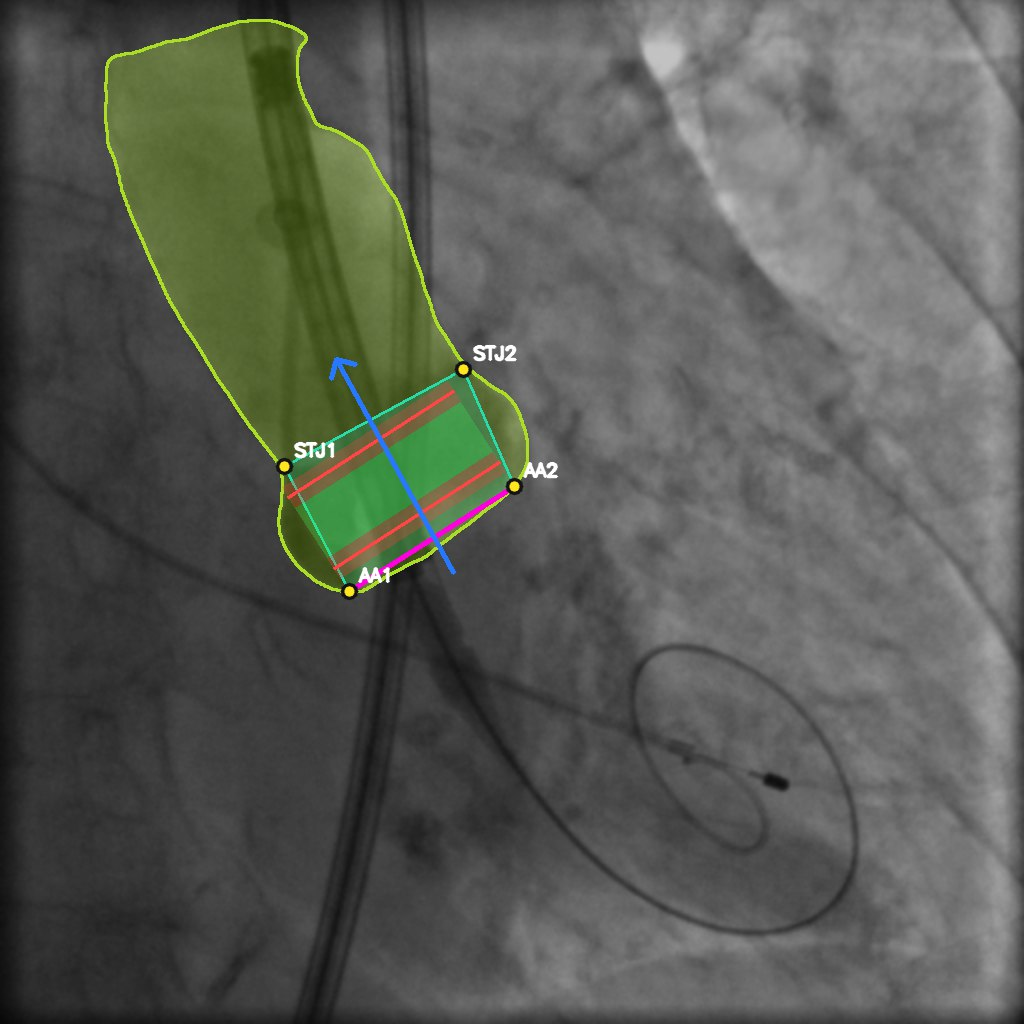
\includegraphics[width=\textwidth]{../figures/60687da9-a664-480a-8eaf-943dd3861d14.jpeg}
        \caption{}
    \end{subfigure}
    \hfill
    \begin{subfigure}[b]{0.48\textwidth}
        \centering
        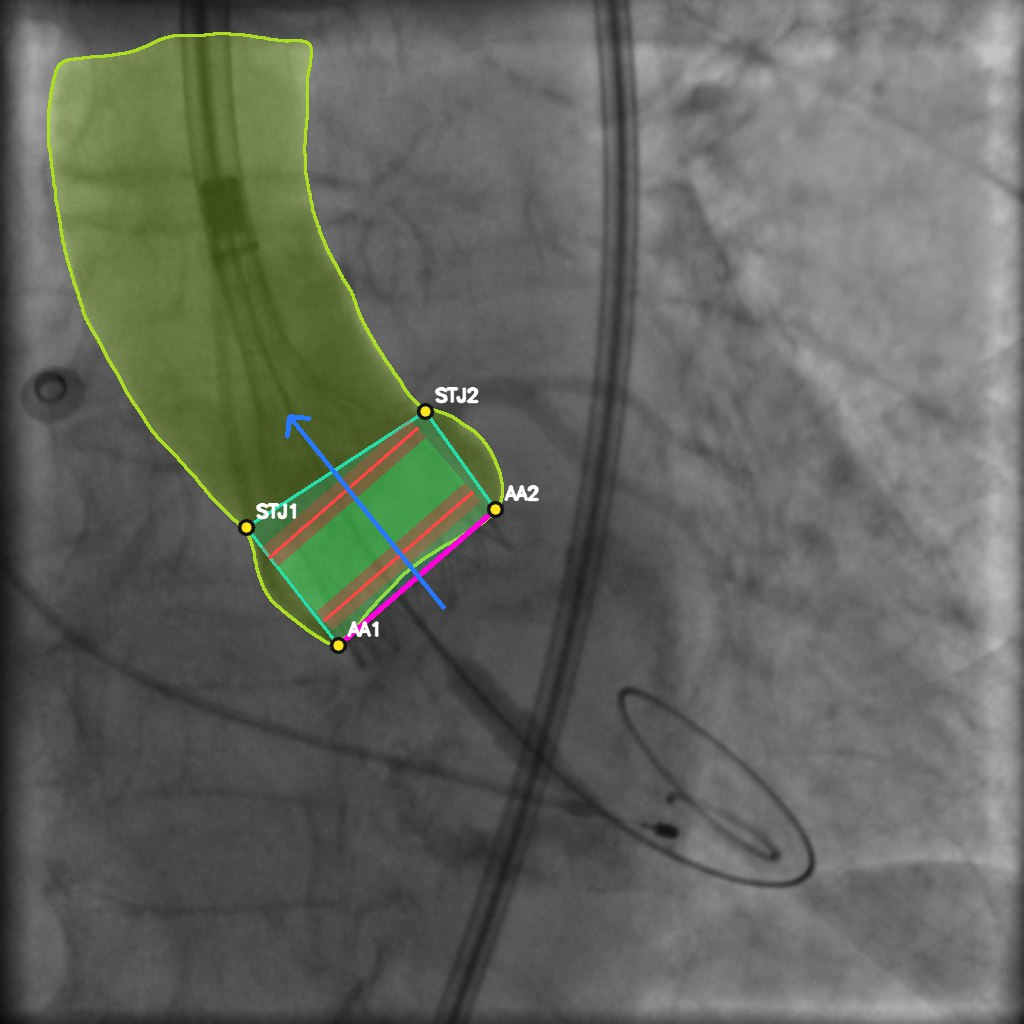
\includegraphics[width=\textwidth]{../figures/fc2fbaf7-c486-4596-b86e-64f8a1a10a86.jpeg}
        \caption{}
    \end{subfigure}
    \caption{Representative BAMNet predictions on intraoperative fluoroscopic frames. The yellow contour and semi-transparent green region denote the predicted aortic root mask. Yellow points correspond to the four predicted landmarks (AA1, AA2, STJ1, STJ2). The blue arrow indicates the estimated aortic axis, and the central geometric overlay illustrates the predicted implantation zone derived from the landmark configuration.}
    \label{fig:bamnet_qualitative}
\end{figure}

\subsection{Patient-level 5-fold cross-validation}\label{subsec:crossval}

To assess robustness, strict patient-level 5-fold cross-validation was performed. Across all five folds, the number of prediction failures remained zero ($n_{\mathrm{pred\_failures}}=0$), indicating stable behavior across different patient subsets. Mean performance across folds reached a Dice score of $0.8974 \pm 0.0237$, an IoU of $0.8257 \pm 0.0329$, a Surface Dice@4~mm of $0.8074 \pm 0.0578$, a median localization error of $8.06 \pm 0.75$~px, and a mean localization error of $11.13 \pm 0.76$~px.

The best segmentation quality was observed on fold~4, where Dice reached 0.9272 and IoU 0.8676, while the best landmark localization was obtained on fold~5, where median and mean errors were 6.97~px and 10.36~px, respectively. Even the least favorable fold remained comparable to the others, supporting good inter-patient generalization.

\begin{table*}[htbp]
\caption{Patient-level 5-fold cross-validation results for BAMNet.}\label{tab:crossval}
\centering
\resizebox{\textwidth}{!}{%
\begin{tabular}{lcccccc}
\toprule
Fold & $n_{samples}$ & Dice & IoU & Surface Dice@4~mm & Median err.\ (px) & Mean err.\ (px) \\
\midrule
1 & 243 & 0.8873 & 0.8053 & 0.7957 & 9.07 & 11.95 \\
2 & 250 & 0.8793 & 0.7930 & 0.7295 & 8.11 & 11.73 \\
3 & 244 & 0.8751 & 0.8087 & 0.7838 & 7.92 & 11.33 \\
4 & 249 & 0.9272 & 0.8676 & 0.8739 & 8.23 & 10.32 \\
5 & 250 & 0.9182 & 0.8538 & 0.8543 & 6.97 & 10.36 \\
Mean $\pm$ SD & 1236 & $0.8974 \pm 0.0237$ & $0.8257 \pm 0.0329$ & $0.8074 \pm 0.0578$ & $8.06 \pm 0.75$ & $11.13 \pm 0.76$ \\
\bottomrule
\end{tabular}}
\end{table*}

\subsection{Landmark-wise localization accuracy}\label{subsec:landmarkwise}

Landmark-specific analysis showed that AA1 was localized most accurately, with a mean error of $8.93 \pm 1.27$~px and a median error of $6.53 \pm 1.29$~px across folds. STJ1 showed similar performance. The most difficult point was AA2, for which the mean error reached $13.79 \pm 1.41$~px and the median error $10.64 \pm 1.48$~px. STJ2 also remained more challenging than AA1 and STJ1. Overall, all four landmarks were localized with clinically relevant precision, but the results suggest greater difficulty for landmarks affected by projection variability, incomplete contrast filling, and partial device overlap.

\begin{table*}[htbp]
\caption{Landmark-wise localization accuracy aggregated over five folds.}\label{tab:landmark_summary}
\centering
\resizebox{0.9\textwidth}{!}{%
\begin{tabular}{lccc}
\toprule
Landmark & Mean err.\ (px, mean $\pm$ SD) & Median err.\ (px, mean $\pm$ SD) & Std.\ err.\ (px, mean $\pm$ SD) \\
\midrule
AA1 & $8.93 \pm 1.27$ & $6.53 \pm 1.29$ & $10.02 \pm 1.38$ \\
AA2 & $13.79 \pm 1.41$ & $10.64 \pm 1.48$ & $12.53 \pm 3.43$ \\
STJ1 & $9.94 \pm 1.28$ & $7.36 \pm 0.75$ & $9.33 \pm 3.22$ \\
STJ2 & $11.89 \pm 2.33$ & $9.09 \pm 2.27$ & $10.72 \pm 2.75$ \\
\bottomrule
\end{tabular}}
\end{table*}

The per-fold breakdown in Table~\ref{tab:landmark_folds} confirms this pattern. AA2 and STJ2 remained the most variable landmarks across folds, whereas AA1 and STJ1 were more stable.

\begin{table*}[htbp]
\caption{Per-fold landmark localization errors for BAMNet.}\label{tab:landmark_folds}
\centering
\resizebox{\textwidth}{!}{%
\begin{tabular}{lcccc}
\toprule
Fold & AA1 mean / median (px) & AA2 mean / median (px) & STJ1 mean / median (px) & STJ2 mean / median (px) \\
\midrule
1 & 10.02 / 8.23 & 15.20 / 12.24 & 10.02 / 7.40 & 12.56 / 8.98 \\
2 & 7.98 / 5.55 & 15.37 / 11.74 & 7.96 / 6.94 & 15.62 / 12.94 \\
3 & 10.34 / 7.37 & 13.22 / 10.15 & 10.66 / 6.34 & 11.06 / 8.27 \\
4 & 8.94 / 6.41 & 12.94 / 10.58 & 9.68 / 7.87 & 9.74 / 8.25 \\
5 & 7.39 / 5.10 & 12.23 / 8.47 & 11.38 / 8.24 & 10.46 / 7.00 \\
\bottomrule
\end{tabular}}
\end{table*}

\subsection{Overall interpretation}\label{subsec:overall}

Taken together, the results indicate that BAMNet is the most balanced model among the tested architectures. It remains competitive with strong segmentation baselines in Dice, IoU, and contour-sensitive metrics while also achieving lower mean landmark localization error than keypoint-only and detection-only approaches. Most importantly, this is achieved within a single model, without the need to chain separate segmentation and detection networks.

\section{Discussion}\label{sec:discussion}

This study introduced BAMNet, a multitask architecture specifically designed for simultaneous dense segmentation of the aortic root and localization of four anatomical landmarks directly on intraoperative fluoroscopic images acquired during TAVI. On the independent validation set, BAMNet achieved Dice~=~0.887, IoU~=~0.805, Surface Dice@4~mm~=~0.796, HD95~=~10.40~mm, and ASSD~=~2.79~mm, together with a mean landmark localization error of 3.16~mm (11.95~px), a median error of 2.39~mm (9.07~px), and an inference speed of 43.9~FPS. In patient-level 5-fold cross-validation, the model remained stable, with Dice~=~$0.897 \pm 0.024$ and mean localization error~=~$11.13 \pm 0.76$~px. These results support the practicality of the approach for intraoperative visual guidance.

\subsection{Technical implications and architectural contribution}\label{subsec:technical}

The overall performance of BAMNet appears to arise not from a single isolated component but from the interaction of multiple design choices. The architecture combines an EfficientNet-V2 encoder, a modified MA-Net decoder, global spatial attention, a dedicated landmark heatmap head, an auxiliary boundary supervision pathway, and coordinate-sensitive feature modulation. Together, these components make it possible to maintain strong segmentation quality while also delivering clinically meaningful landmark coordinates.

The ablation study therefore focused on the components present in the final architecture: PositionAttention in the decoder, Coordinate Attention in the landmark branch, deep-decoder feature fusion, boundary guidance and boundary loss, and the soft-argmax temperature schedule. This analysis was designed to assess how global spatial context, coordinate-aware feature modulation, auxiliary boundary supervision, and heatmap-to-coordinate conversion affect the balance between segmentation quality and landmark localization accuracy. The overall ranking of these architectural variants is summarized in Fig.~\ref{fig:ablation_summary}. From a deployment perspective, the main practical benefit is that BAMNet removes the need to run two separate models at inference time. The reported throughput of 43.9~FPS on an NVIDIA RTX4070 is compatible with real-time fluoroscopic assistance.

\begin{figure}[htbp]
\centering
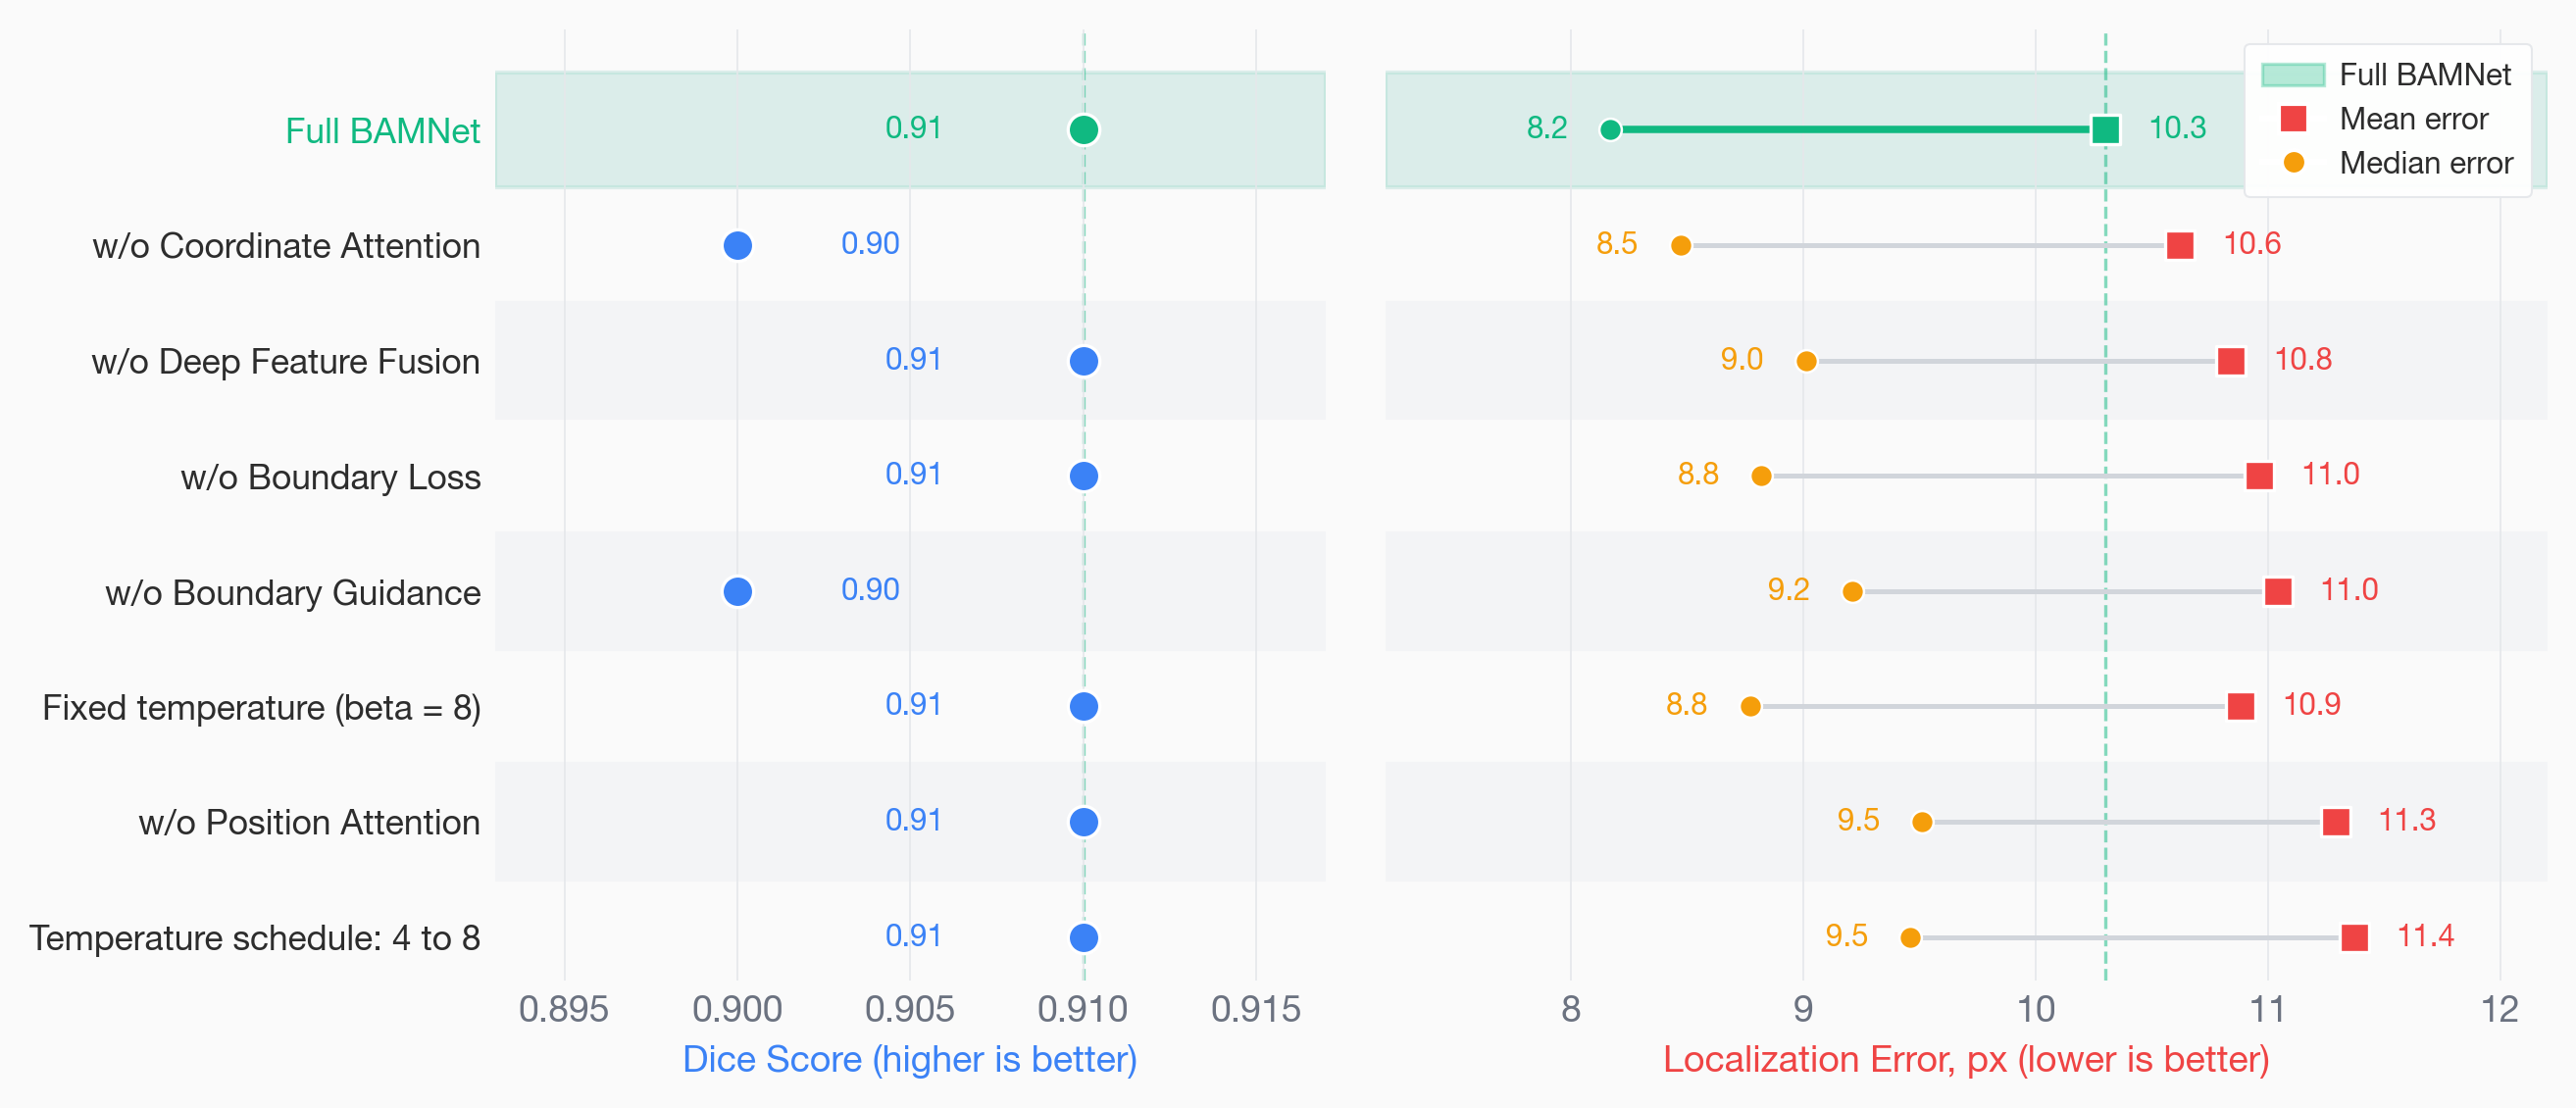
\includegraphics[width=\textwidth]{../figures/ablation_summary.png}
\caption{Summary of the BAMNet ablation study across the main architectural variants. The figure highlights how global spatial attention, coordinate-aware modulation, feature fusion, boundary-related supervision, and the soft-argmax configuration affect the balance between segmentation quality and landmark localization accuracy.}
\label{fig:ablation_summary}
\end{figure}

\subsection{Clinical relevance}\label{subsec:clinical}

Producing both an aortic root mask and key landmark coordinates in one pass has direct clinical relevance. One potential benefit is a reduced need for repeated contrast aortography. Although the present study did not measure the volume of contrast saved directly, continuous anatomical overlay on fluoroscopy could lower the number of repeat contrast series and may therefore be particularly useful in patients with chronic kidney disease or elevated risk of contrast-induced nephropathy \cite{dangas2020_tavi,yamamoto2021_tavi}.

A second important aspect is valve positioning accuracy. Even modest implantation-depth deviations are associated with paravalvular regurgitation, coronary obstruction, and conduction abnormalities requiring permanent pacing \cite{pibarot2021_pvl,jilaihawi2022_coronary,kammler2016_implantdepth}. In the present study, the median localization error on the validation set was 2.39~mm and the mean error was 3.16~mm. These values already approach a range that is potentially useful for visual assistance. The more conservative cross-validation results, with median and mean errors of $8.06 \pm 0.75$~px and $11.13 \pm 0.76$~px, still indicate reproducible performance suitable for stable anatomical overlay.

The third clinical implication concerns radiation burden. If the model reduces the need for additional angiographic runs, it may also reduce cumulative exposure for both the patient and the operating staff. Although radiation dose was not measured directly here, the task formulation is aligned with the ALARA principle and with the broader objective of safer intraoperative guidance.

\subsection{Toward robot-assisted and autonomous TAVI}\label{subsec:robotic}

One of the most promising applications of BAMNet is robot-assisted or visually assisted TAVI. Such systems require more than segmentation alone: they need temporally stable landmark coordinates that can support navigation, motion compensation, and possibly closed-loop control. This is why the multitask output of BAMNet is substantially more valuable than isolated segmentation in this context.

The current validation-set median landmark error of 9.07~px (2.39~mm) and mean error of 11.95~px (3.16~mm) are clinically meaningful for visual assistance and provide a realistic baseline for more advanced scenarios. With the addition of temporal modeling, sequence-level filtering, and explicit compensation for cardiac and respiratory motion, further reductions in coordinate instability may be achievable. The fact that the model reasons over both local appearance and global spatial context may also make it more robust when the aortic root is partially obscured by the delivery system or catheters, which is precisely the setting where simple tracking or segmentation approaches often fail \cite{smits2025_autonomous,clinicaltrials_nct07152574}.

\subsection{Limitations}\label{subsec:limitations}

This study has several limitations. First, despite the relatively large dataset of 2,925 images from 83 patients, the material remains single-center. External validation on data from other centers, fluoroscopy systems, and valve types is needed before broader generalization can be claimed. Second, all analysis was performed in a frame-wise setting; temporal consistency across neighboring frames was not studied. That limitation is particularly important for future integration into robotic systems.

Third, while the observed localization errors are promising for visual assistance, fully autonomous control would likely require higher precision together with predictable temporal stability. Finally, we have not yet performed a prospective clinical evaluation of the effect of BAMNet on procedure duration, contrast volume, radiation dose, or complication rates. The present results should therefore be interpreted as a technological proof of feasibility rather than definitive evidence of clinical benefit.

\subsection{Future directions}\label{subsec:future}

Several natural extensions follow from the present work. The first is a move toward multi-frame modeling with temporal loss functions or recurrent/video architectures in order to stabilize landmark tracking throughout the cardiac cycle. A second direction is biplane fluoroscopy with 3D reconstruction of anatomical landmarks. A third is prospective clinical evaluation with explicit measurement of positioning accuracy, procedure duration, contrast use, and radiation exposure. Finally, an important translational direction is integration of BAMNet into a human-machine guidance loop for navigation and robot-assisted TAVI.

\section{Conclusion}\label{sec:conclusion}

BoundaryAwareMAnet (BAMNet) is a new multitask deep learning architecture for simultaneous segmentation of the aortic root and localization of four key anatomical landmarks on intraoperative fluoroscopic images acquired during TAVI. On an independent validation set, the model achieved Dice~=~0.887, IoU~=~0.805, Surface Dice@4~mm~=~0.796, HD95~=~10.40~mm, ASSD~=~2.79~mm, and a mean landmark localization error of 3.16~mm (11.95~px), while maintaining real-time inference at 43.9~FPS.

In patient-level 5-fold cross-validation, BAMNet remained stable, with Dice~=~$0.897 \pm 0.024$, IoU~=~$0.826 \pm 0.033$, Surface Dice@4~mm~=~$0.807 \pm 0.058$, median localization error~=~$8.06 \pm 0.75$~px, and mean localization error~=~$11.13 \pm 0.76$~px. By combining high-quality segmentation and clinically useful landmark localization in one pass, BAMNet offers a practical foundation for standard TAVI guidance and a direct step toward future semi-automated and robot-assisted valve implantation workflows.

\backmatter

\bmhead{Supplementary information}

No supplementary files are included in this manuscript version.

\bmhead{Acknowledgements}

TODO.

\section*{Declarations}

\section*{Funding}

This study was supported by the Russian Science Foundation under Grant No.~24-19-00084, titled \textit{``Robotic System for Medical Instrument Delivery with Integrated Intelligent Information Processing''}. For more information, please visit \href{https://rscf.ru/project/24-19-00084/}{https://rscf.ru/project/24-19-00084/}.

\section*{Data Availability Statement}

All essential components of the study, including curated source code, data, and trained models, have been made publicly available:

\begin{itemize}
\item \textbf{Source code:} \url{https://github.com/Nikita75699/segmentation_tavi}
\item \textbf{Dataset:} \url{https://doi.org/10.5281/zenodo.15094600}
\item \textbf{Models:} \url{https://doi.org/10.5281/zenodo.15106413}
\end{itemize}

\section*{Conflict of Interest Statement}

Authors declare that the research was conducted in the absence of any commercial or financial relationships that could be construed as a potential conflict of interest.

\noindent\textbf{Ethics approval and consent to participate} TODO.

\noindent\textbf{Consent for publication} TODO.

\noindent\textbf{Data availability} See the Data Availability Statement above.

\noindent\textbf{Materials availability} TODO.

\noindent\textbf{Code availability} See the Data Availability Statement above.

\section*{Author Contributions}

NL: Conceptualization, Data curation, Formal analysis, Investigation, Methodology, Software, Supervision, Validation, Visualization, Writing--original draft, Writing--review and editing. OG: Formal analysis, Investigation, Methodology, Software, Validation, Visualization, Writing--review and editing. YK: Data curation, Formal analysis, Visualization, Writing--review and editing. EV: Data curation, Writing--review and editing. MC: Conceptualization, Funding acquisition, Project administration, Resources, Supervision, Writing--review and editing. VD: Methodology, Resources, Validation, Writing--review and editing, Supervision.

\bibliography{bamnet}

\end{document}
